\documentclass[documentation]{FEIstyle} % Options documentation is for custom document - QWeuroR

% Author of the thesis
\FEIauthor{\shortstack[r]{Bc. Samuel Kopp\\Bc. Jakub Janega}}

% Evidence number
\FEIregNr{FEI-xxxx-xxxx}

% Title
\FEItitle{Projekt - Riadenie mobilných robotov}
\FEItitleEn{Documentation Template in \LaTeX}

% Date
\FEIdate{15}{5}{2026}

% Keywords
\FEIkeywords{dokumentácia, šablóna, \LaTeX, formátovanie textu, citácie}
\FEIkeywordsEn{Documentation, template, \LaTeX, text formatting, citations}

% Further details
\FEIstudyProgramme{Robotika a kybernetika}
\FEIstudyProgrammeEn{Study program in English}
\FEIstudyField{názov študijného odboru}
\FEIstudyFieldEn{Field of the study in English}
\FEItrainingWorkplace{Názov školiaceho pracoviska}
\FEItrainingWorkplaceEn{Training Work place}

% Course information (required for seminar paper option)
\FEIcourseTag{I-RMR}         % Course code
\FEIcourse{Riadenie mobilných robotov}       % Course name in Slovak
\FEIcourseEn{Course name}        % Course name in English
\FEIlecturer{prof. Ing. František Duchoň, PhD.}    % Lecturer's name
\FEITA{Ing. Martin Dekan, PhD.}           % Teaching assistant's name

% Supervisor
\FEIsupervisor{tituly Meno Priezvisko, tituly}

% Consultant
% -- if there is none, comment out the next line
\FEIconsultant{tituly Meno Priezvisko, tituly}

% Glossaries -- terms and abbreviations.
% If you use automatic glossaries,
% uncomment the next line.
%\FEIglossaries{includes/glossary}

% Bibliography database file
% \bibliography{includes/bibliography.bib}

\begin{document}

%%%%%%%%%%%%%%%%%%
%%              %%
%% FRONT MATTER %%
%%              %%
%%%%%%%%%%%%%%%%%%
\frontmatter

\FEIpdfInfo
% \FEIcover % turned off for documentation type - QWeuroR
\FEItitlePage
% 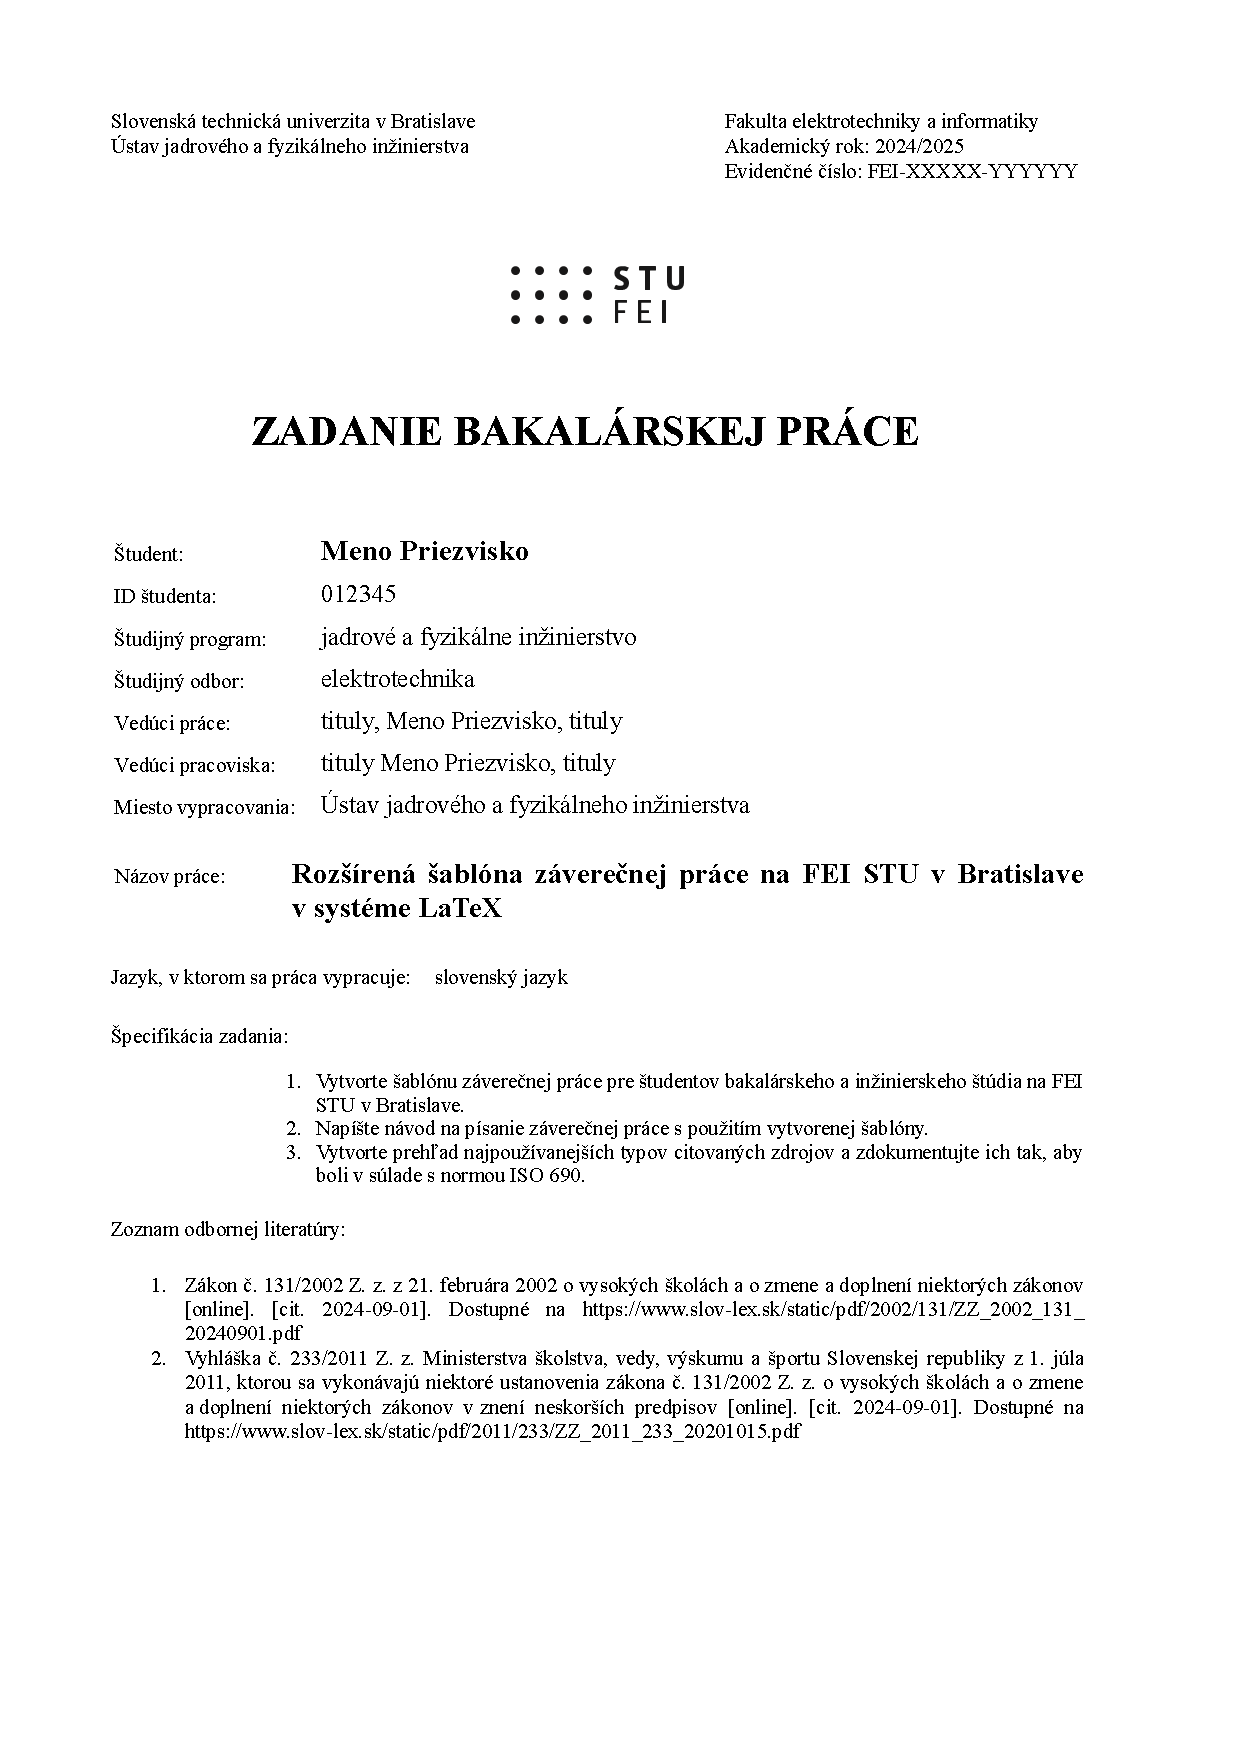
\includepdf[pages=-]{includes/assignment.pdf}
%  \FEIthanks{includes/thanks} % turned off for documentation type - QWeuroR
% \FEIabstract{includes/abstract} % turned off for documentation type - QWeuroR
% \FEIabstractEn{includes/abstractEN} % turned off for documentation type - QWeuroR
\FEIcontent
%\FEIlistOfFiguresAndTables

%% List of units and abbreviations
%%
%% Choose the method of typesetting the list of
%% units and abbreviations.
%% Uncomment only one of the two lines below!

%% METHOD 1:
%% ---------
%% Automatically generated and sorted list of
%% abbreviations with hyperlinks from the text.
%% Edit includes/glossary.tex.
%\FEIlistOfGlossaries
%% METHOD 2:
%% ---------
%% Manual list -- must be manually filled and sorted,
%% does not make hyperlinks from the text.
%% Edit includes/manual_glossary.tex.
% \FEImanualListOfGlossaries{includes/manual_glossary} % turned off for documentation type - QWeuroR

%% Lists of algorithms and listings
% \FEIlistOfAlgorithms % turned off for documentation type - QWeuroR
% \FEIlistOfListings % turned off for documentation type - QWeuroR

%%%%%%%%%%%%%%%%%
%%             %%
%% MAIN MATTER %%
%%             %%
%%%%%%%%%%%%%%%%%
\mainmatter

% \FEIintroduction{includes/introduction}
\FEIcore{includes/core}
% \FEIconclusion{includes/conclusion}

%% Uncomment only if the document is writen in english
%\FEIresume{includes/resume}

%%%%%%%%%%%%%%%%%%
%%              %%
%% Bibliography %%
%%              %%
%%%%%%%%%%%%%%%%%%
% \FEIbibliography
%% AI Declaration
%  \FEIaiDeclaration{includes/ai_declaration} % turned off for documentation type - QWeuroR

%%%%%%%%%%%%%%%%%%
%%              %%
%% BACK MATTER  %%
%%              %%
%%%%%%%%%%%%%%%%%%
\backmatter

% ____ turned off for documentation type - QWeuroR
% %% Attachment A
% \FEIappendix{Algoritmus\label{att:algorithms}}{includes/attachmentA}

% %% Attachment B
% \FEIappendix{Výpis dlhého kódu\label{att:listings}}{includes/attachmentB}

% %% Attachment C
% \FEIappendix{Slovníček pojmov\label{att:dictionary}}{includes/attachmentC}

% %% Attachement D
% %\FEIappendix{Súborová štruktúra projektu\label{att:files}}{includes/attachmentD}
% ____ turned off for documentation type - QWeuroR

\end{document}
